\subsection{Commit Extractor Plug-ins}
\label{sec:CommitExtractorPlugins}
\ToDo{
\begin{itemize}
	\item Definition and usage of plug-in-specific configuration parameters in introduction of parent section?
	\item Purpose of plug-in type
	\item Typical input
	\item Realization via implementation of abstract class along example
	\begin{itemize}
		\item The three extraction variants
		\item Creating data model element instances
		\item Passing extracted elements to analyses
	\end{itemize}
	\item Passing extracted elements to analyses as transition to Section~\ref{sec:CommitAnalyzerPlugins}
\end{itemize}
}
A commit extractor plug-in is responsible for extracting commit information from a software repository and providing this information for an analysis. Therefore it has to create instances of the \texttt{Commit} and \texttt{ChangedArtifact} classes described in Section~\ref{sec:DataModel} and add these instances to the internal \texttt{CommitQueue}. This queue represents the actual connection between commit extractors and analyzers. It is accessible through an attribute of the \texttt{AbstractCommitExtractor} class, which each commit extractor has to extend. Figure~\ref{fig:AbstractCommitExtractorClass} presents this abstract class as well as the extractor-specific commit queue interface.

\begin{figure}[ht] % t für top, b = bottom, h = here
	\centering
		%trim={<left> <lower> <right> <upper>}
		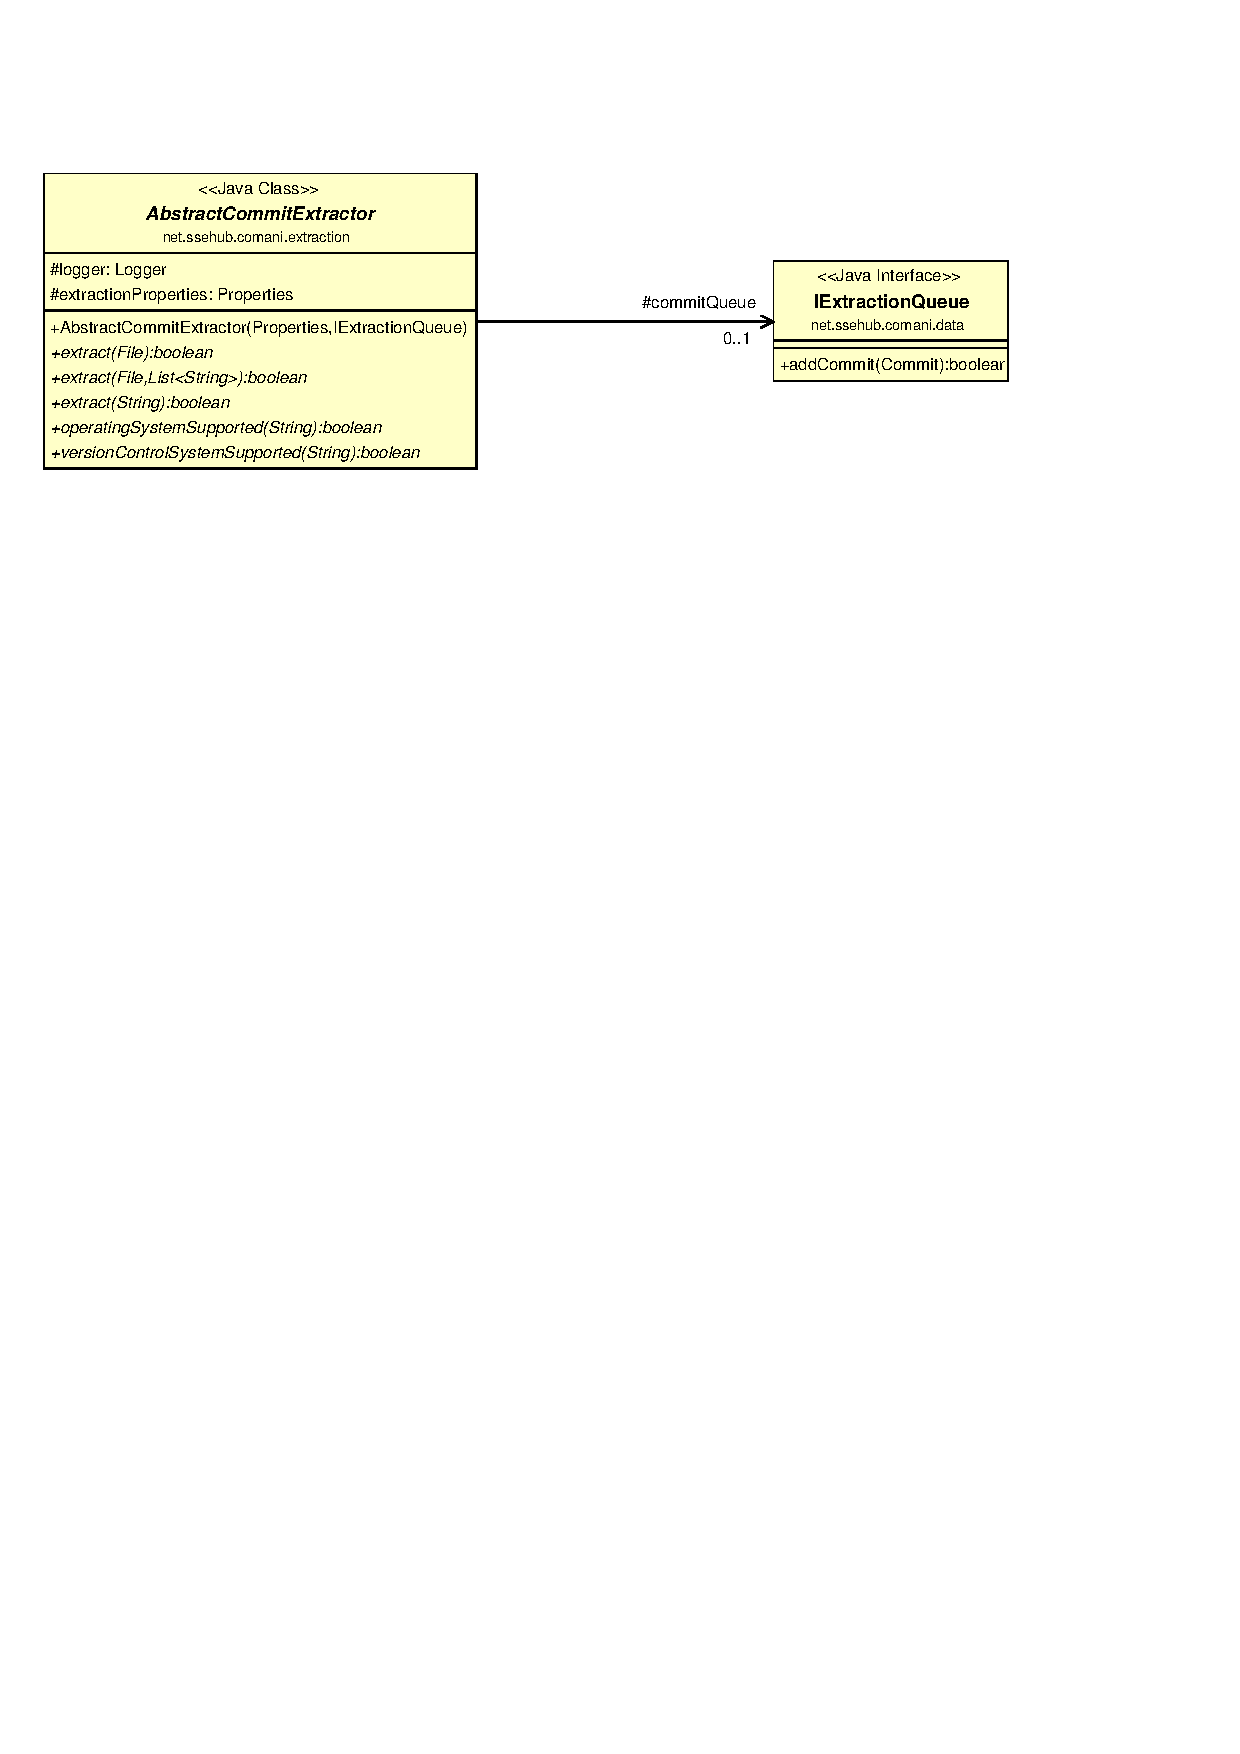
\includegraphics[width=\columnwidth,trim={0,7cm 21,7cm 3,9cm 2,9cm},clip]{inserts/comani_abstract_commit_extractor.pdf}
  \caption{\thetool{} \texttt{AbstractCommitExtractor} class}
	\label{fig:AbstractCommitExtractorClass}
\end{figure}

Each commit extractor inherits three attributes: the infrastructure-wide logger, the extraction properties, and the commit queue as shown in Figure~\ref{fig:AbstractCommitExtractorClass}. The \texttt{logger} provides multiple methods for logging general information about the extraction process, warning, error, and debug messages. The amount of information actually shown, e.g., on the command line, depends on the defined log-level in the configuration file (cf. Section~\ref{sec:Execution}). The \texttt{extractionProperties} include all configuration parameters, which start with the prefix ``\texttt{extraction.}'', a property providing the name of the operating system on which the extractor currently runs, and a property for the version control system as specified by the respective configuration parameter in the configuration file (cf. Section~\ref{sec:Execution}). The \texttt{commitQueue} enables the transfer of extracted commits to an analysis. It only provides a single method, which accepts a single \texttt{Commit} instance as a parameter. Hence, the extraction algorithms have to call this method for each extracted commit individually.

Figure~\ref{fig:AbstractCommitExtractorClass} also shows that a commit extractor has to implement a constructor, which accepts a properties and a particular extraction queue instance as parameters, as well as a set of methods for extracting commits and checking whether it is executable in the current environment. Listing~\ref{lst:CommitExtractorBlueprint} introduces a blueprint of a commit extractor, which implements all these required elements.

\ToDo{
Explain how to guarantee addition of commit to queue:
  while (!commitQueue.addCommit(commit)) {
      logger.log(ID, "Waiting to add commit to queue", null, MessageType.DEBUG);
  }
}

\begin{figure}[ht]
	\centering
		\lstinputlisting[caption={Blueprint of a \thetool{} commit extractor main class},label=lst:CommitExtractorBlueprint,basicstyle=\small,language=Java]{inserts/CommitExtractor.java}
\end{figure}

This blueprint represents a starting point for each new extractor by implementing the necessary algorithms as follows:

\begin{enumerate}
	\item \textit{Constructor}: creates a new instance of the commit extractor and, hence, has to call its parent class’ constructor by passing the constructor parameters of the new extractor. Further actions for setting up the particular commit extractor can be performed here as well, which may also throw \texttt{ExtractionSetupException}s, if the setup fails. Listing~\ref{lst:CommitExtractorBlueprint} shows the constructor in Lines 16 to 22 including the usage of the \texttt{logger}, which informs the user about its creation (Line 20).
	\item \textit{Extraction methods}: realize the three extraction variants as introduced in Section~\ref{sec:Overview}. Each method in the Lines 25 to 41 returns a Boolean value indicating whether the particular extraction variant was successful (\texttt{true}) or not (\texttt{false}). In the latter case, the user is automatically informed about an extraction error indicating that either there are no analysis results or the results may potentially be incorrect. The individual methods have the following purpose:
	\begin{enumerate}
		\item \texttt{extract (File repository)}: extracts all commits of the given software repository. The \texttt{repository} parameter identifies the directory specified as input (\texttt{extraction.input}) in the configuration file (cf. Section~\ref{sec:Execution}), which is typically the root directory of a software repository. The particular way of interacting with the supported type of repository depends on the commands and capabilities provides by the version control system.
		\item \texttt{extract (File repository, List<String> commitList)}: extracts only those commits of the given software repository, which are part of the given commit list. While the \texttt{repository} parameter provides the same information as for the method above, the \texttt{commitList} parameter contains a set of commit numbers (or hashes), which enable to extraction of the respective commits. However, this method is only called if a commit list is defined via the corresponding configuration parameter in the configuration file.
		\item \texttt{extract (String commit)}: transforms the given information representing the content of a particular commit into a commit of the internal data model. This method is only called in the interactive mode of \thetool{}, in which the given string is passed directly as a command line argument.
	\end{enumerate}
	\item \textit{Support check methods}: realize the opportunity to restrict the application of a commit extractor to a particular operating system and version control system. In particular, this is important, if, for example, an extractor relies on a third-party library, which is only available for Windows, or if the extractor cannot process other commits than those of a Git repository. A missing support yields a \texttt{ExtractionSetupException} during the creation of an instance of the extractor by the infrastructure, which terminates the entire tool. Each method in Lines 44 to 54 returns a Boolean value indicating whether the extractor supports the respective system (\texttt{true}) or not (\texttt{false}):
	\begin{enumerate}
		\item \texttt{operatingSystemSupported(String os)}: checks whether the extractor supports the given operating system. The \texttt{os} parameter provides the operating system in the format of \texttt{System.getProperty(``os.name'')}\footnote{\url{https://docs.oracle.com/javase/tutorial/essential/environment/sysprop.html}}.
		\item \texttt{versionControlSystemSupported(String vcs)}: checks whether the extractor supports the given version control system. The \texttt{vcs} parameter provides the version control system as defined by the \texttt{core.version\_control\_system} configuration parameter in the configuration file.
	\end{enumerate}
\end{enumerate}

\ToDo{
\begin{enumerate}
	\item Explain in detail how to extract commits and pass them to the queue using an excerpt of the git commit extractor
	\item Explain how to define and use custom configuration parameters for an extractor
	\item Add the quick steps for extractor project creation as in the Word doc
\end{enumerate}
}
